\documentclass[aspectratio=169]{beamer}
\usepackage[utf8]{inputenc}
\usepackage[T1]{fontenc}
\usepackage[brazil]{babel}
\usepackage{ragged2e}
\usepackage{booktabs}
\usepackage{verbatim}
\usetheme{AnnArbor}
\usecolortheme{orchid}
\usefonttheme[onlymath]{serif}
\usepackage{listings}

\lstset{language=C,
	backgroundcolor=\color{green!10},
	basicstyle=\ttfamily,
	keywordstyle=\color{blue}\ttfamily,
	stringstyle=\color{red}\ttfamily,
	commentstyle=\color{green}\ttfamily,
	morecomment=[l][\color{magenta}]{\#}
}

\AtBeginSection[]{
  \begin{frame}
  \vfill
  \centering
  \begin{beamercolorbox}[sep=8pt,center,shadow=true,rounded=true]{title}
    \usebeamerfont{title}\insertsectionhead\par%
  \end{beamercolorbox}
  \vfill
  \end{frame}
}

\title[\sc{Complexidade de Algoritmos}]{Complexidade de Algoritmos}
\author[Roland Teodorowitsch]{Roland Teodorowitsch}
\institute[ALEST I - EP - PUCRS]{Algoritmos e Estruturas de Dados I - Escola Politécnica - PUCRS}
\date{31 de julho de 2023}

\begin{document}
\justifying

%-------------------------------------------------------
\begin{frame}
	\titlepage
\end{frame}

%=======================================================
\section{Apresentação}

%-------------------------------------------------------
\begin{frame}\frametitle{Leituras Recomendadas}

\begin{columns}[T]
\begin{column}{0.15\linewidth}
\vspace{-3mm}
\begin{figure}[h]
	\centering
	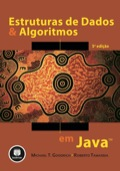
\includegraphics[height=0.3\paperheight]{pucrs-ec-poo-unidade_01-complexidade_de_algoritmos-laminas-livro_goodrich.jpg}
\end{figure}
\end{column}
\begin{column}{0.85\linewidth}
\vspace{3mm}
\textbf{Capítulo 4}\\
\scriptsize{GOODRICH, Michael T.; TAMASSIA, Roberto. \textbf{Estruturas de dados e algoritmos em Java}. Tradução: Bernardo Copstein. 5. ed. Porto Alegre: Bookman, 2013. xxii, 713 p. E-book. ISBN 9788582600191. Tradução de: Data Structures and Algorithms in Java, 5th Edition. Disponível em: \textless{}\url{https://integrada.minhabiblioteca.com.br/\#/books/9788582600191/}\textgreater{}. Acesso em: 01 ago. 2023.}
\end{column}
\end{columns}

\vspace{5mm}

\begin{columns}[T]
\begin{column}{0.15\linewidth}
\vspace{-3mm}
\begin{figure}[h]
	\centering
	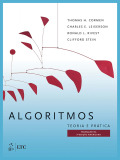
\includegraphics[height=0.3\paperheight]{pucrs-ec-poo-unidade_01-complexidade_de_algoritmos-laminas-livro_cormen.jpg}
\end{figure}
\end{column}
\begin{column}{0.85\linewidth}
\vspace{3mm}
\textbf{Capítulo 3}\\
\scriptsize{CORMEN, Thomas \emph{et al}. \textbf{Algoritmos - Teoria e Prática}. Tradução: Arlete Simille Marques. Rio de Janeiro: Grupo GEN, 2012. E-book. ISBN 9788595158092. Tradução de: Introduction to Algorithms, 3rd ed. Disponível em: \textless{}\url{https://integrada.minhabiblioteca.com.br/\#/books/9788595158092/}\textgreater{}. Acesso em: 01 ago. 2023.}
\end{column}
\end{columns}

\end{frame}

%-------------------------------------------------------
\begin{frame}\frametitle{Sumário}
\begin{itemize}
	\item Complexidade e análise de algoritmos
	\item Contando o tempo
	\item Contagem de operações
	\item Funções
\end{itemize}
\end{frame}

%=======================================================
\section{Complexidade e análise de algoritmos}

%-------------------------------------------------------
\begin{frame}\frametitle{Complexidade e análise de algoritmos}
\begin{itemize}
	\item  No desenvolvimento de uma aplicação tem-se como objetivo projetar ``boas'' estruturas de dados e ``bons'' algoritmos
	\begin{itemize}
		\item Otimizados
		\item Simples
	\end{itemize}
	\item Como saber se um algoritmo é eficiente?
\end{itemize}
\end{frame}

%-------------------------------------------------------
\begin{frame}\frametitle{Análise de Algoritmos}
\begin{itemize}
	\item Estudo das características de desempenho de um determinado algoritmo
	\begin{itemize}
		\item O espaço ocupado é uma característica de desempenho
		\item O tempo gasto na execução é outra característica de desempenho
	\end{itemize}
\end{itemize}
\end{frame}

%-------------------------------------------------------
\begin{frame}\frametitle{Complexidade de Algoritmos}
\begin{itemize}
	\item A \textbf{complexidade de um algoritmo} é a \textbf{medida do consumo de recursos} de que o algoritmo necessita durante a sua execução
	\begin{itemize}
		\item Tempo de processamento
		\item Memória ocupada
		\item Largura de banda de comunicação
		\item Hardware necessário
		\item etc.
	\end{itemize}
\end{itemize}
\end{frame}

%=======================================================
\section{Contando o tempo}

%-------------------------------------------------------
\begin{frame}\frametitle{Tempo de processamento}
\begin{itemize}
	\item Depende de uma série de fatores: \emph{hardware}, \emph{software}, tamanho e tipo da entrada de dados
	\item Algoritmo: tempo de execução (ms) X tamanho da entrada de dados (n)
	\begin{figure}[h]
		\centering
		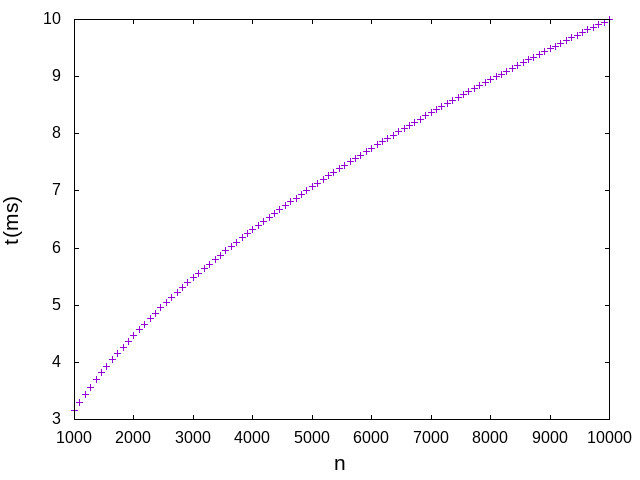
\includegraphics[height=0.6\paperheight]{pucrs-ec-poo-unidade_01-complexidade_de_algoritmos-laminas-grafico.jpg}
	\end{figure}
\end{itemize}
\end{frame}

%-------------------------------------------------------
\begin{frame}[fragile]\frametitle{Medindo o tempo}
\begin{itemize}
	\item Em Java, \texttt{System.currentTimeMillis()} retorna o tempo em milissegundos (ms)
{\scriptsize
\begin{lstlisting}
long antes = System.currentTimeMillis();
// algoritmo a ser medido...
long ms = System.currentTimeMillis() - antes;
\end{lstlisting}}
	\item Em Java, \texttt{System.nanoTime()} retorna o tempo em nanossegundos (ns)
{\scriptsize
\begin{lstlisting}
long antes = System.nanoTime();
// algoritmo a ser medido...
long ns = System.nanoTime() - antes;
\end{lstlisting}}
	\item Em C, no Unix, pode-se usar \texttt{gettimeofday()} (incluir \texttt{<sys/time.h>})
{\scriptsize\begin{lstlisting}
struct timeval antes, depois;
gettimeofday(&antes, NULL);
// algoritmo a ser medido...
gettimeofday(&depois, NULL);
unsigned long ms = (depois.tv_sec  - antes.tv_sec) * 1000000 +
                    depois.tv_usec - antes.tv_usec;
\end{lstlisting}}

\end{itemize}
\end{frame}

\begin{comment}
120 420 6x467


 Exemplo: tempo de execução para algoritmo
bubble sort

%-------------------------------------------------------
\begin{frame}\frametitle{Contando o tempo}
\begin{itemize}
	\item Outro exemplo: busca sequencial em um arranjo
public static int localiza(int[] dados, int valor) {
for(int pos=0; pos<dados.length; pos++)
if(valor == dados[pos])
return pos;
return -1;
}
◼
 O método recebe um arranjo e um valor a ser
localizado, e retorna a posição do valor no arranjo
(ou -1 se não achar).


%-------------------------------------------------------
\begin{frame}\frametitle{Contando o tempo}
\begin{itemize}
	\item Para "enxergar" a complexidade, deve-se executar o método várias vezes, com um arranjo cada vez maior:
public static void main(String[] args) {
int[] lista;
for(int total=1_000_000; total<8_000_000; total+=10000){
lista = new int[total];
for(int pos=0; pos<total; pos++)//preenche o arranjo
lista[pos] = pos;
}
}
long antes = System.currentTimeMillis();
int loc = localiza(lista, total-1);//pior caso:último elem
long depois = System.currentTimeMillis();
long tempo = depois - antes;
System.out.println(total + " " + tempo); // saída
// total de elementos x tempo

%-------------------------------------------------------
\begin{frame}\frametitle{Contando o tempo}
\begin{itemize}
	\item A partir da saída do
programa:
1000000 5
1010000 1
1020000 2
...
◼
Gráfico da
quantidade de
dados de entrada x
tempo.
◼
Qual a origem da
variação no tempo
de execução?


%-------------------------------------------------------
\begin{frame}\frametitle{Contando o tempo}
\begin{itemize}
	\item Análise da eficiência de um algoritmo
◼
 Medir o tempo depende de hardware e software
(sistema operacional, por exemplo)
◼
 Alternativa?
Contar o número de operações
(atribuição, operação
aritmética, comparação, etc.)

\end{comment}

%=======================================================
\section{Contagem de operações}


%-------------------------------------------------------
\begin{frame}\frametitle{Análise de algoritmos}
\begin{itemize}
	\item Não pode considerar o tempo de execução
	\item Deve ser feita diretamente sobre o pseudocódigo de alto nível
	\item Consiste em contar quantas \textbf{operações primitivas} são executadas
	\begin{itemize}
		\item Operação primitiva: instrução de baixo nível com um tempo de execução constante
	\end{itemize}
	\item Assume-se que os tempos de execução de operações primitivas diferentes são similares
\end{itemize}
\end{frame}

%-------------------------------------------------------
\begin{frame}\frametitle{Operações primitivas}
\begin{itemize}
	\item Atribuição de valores a variáveis
	\item Chamadas de métodos
	\item Operações aritméticas (por exemplo, adição de dois números)
	\item Comparação de dois números
	\item Acesso a um arranjo
	\item Retorno de um método
\end{itemize}
\end{frame}

%-------------------------------------------------------
\begin{frame}[fragile]\frametitle{Exemplo 1}
\begin{itemize}
	\item Contar o número de operações para atribuir para cada posição v[i] de um arranjo unidimensional o resultado de i*2
\begin{verbatim}
v[0..10] : inteiro
for (i = 0; i < v.comprimento; i++)
    v[i] = i * 2
\end{verbatim}
	\pause
	\item Operação (multiplicação, atribuição e acesso as posições do arranjo): \textbf{n vezes (n = 10)}
	\pause
	\begin{figure}[h]
		\centering
		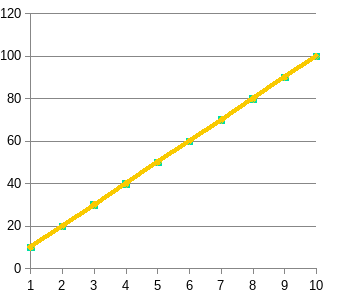
\includegraphics[height=0.4\paperheight]{pucrs-ec-poo-unidade_01-complexidade_de_algoritmos-laminas-grafico2.png}
	\end{figure}
\end{itemize}
\end{frame}

%-------------------------------------------------------
\begin{frame}[fragile]\frametitle{Exemplo 2}
\begin{itemize}
	\item Contar o número de operações para atribuir para cada posição m[i,j] de um arranjo bidimensional o resultado de i*j
\begin{verbatim}
m[0..10][0..10] : inteiro
for (i=0; i<m.comprimento; i++)
    for (j=0; j<m[i].comprimento; j++)
        m[i][j] = i * j
\end{verbatim}
	\pause
	\item Operação (multiplicação, atribuição e acesso as posições do arranjo): \textbf{n*n vezes (n = 10)}
	\pause
	\begin{figure}[h]
		\centering
		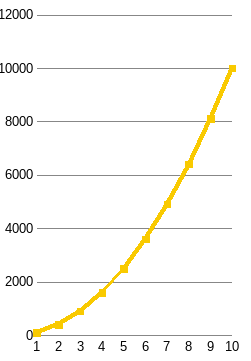
\includegraphics[height=0.35\paperheight]{pucrs-ec-poo-unidade_01-complexidade_de_algoritmos-laminas-grafico3.png}
	\end{figure}
\end{itemize}
\end{frame}


%-------------------------------------------------------
\begin{frame}[fragile]\frametitle{Exercícios (1/2)}
Implementar e contar o número de operações das funções listadas a seguir.
\begin{columns}[T]
\begin{column}{0.5\linewidth}
\begin{enumerate}
	\item
{\small
\begin{verbatim}
int f1(n)
    r=0
    for (i=1; i<n; i++)
        r = r + 1
    return r
\end{verbatim}
}
	\item
{\small
\begin{verbatim}
int f2(n)
    r=0
    for (i=1; i<n; i++)
        for (j=i+1; j<n; j++)
            r = r + 2
    return r
\end{verbatim}
}
\end{enumerate}
\end{column}
\begin{column}{0.5\linewidth}
\begin{enumerate}
\setcounter{enumi}{2}
	\item
{\small
\begin{verbatim}
int f3(n)
    cont=0
    for (i=1; i<n; i++)
        for (j=1; j<n; j++)
            print i*j
            cont++
     return cont
\end{verbatim}
}
\end{enumerate}
\end{column}
\end{columns}
\end{frame}

%-------------------------------------------------------
\begin{frame}[fragile]\frametitle{Exercícios (2/2)}
\begin{columns}[T]
\begin{column}{0.5\linewidth}
\begin{enumerate}
\setcounter{enumi}{3}
	\item
{\small
\begin{verbatim}
int f4(n)
    r=0
    for (i=1; i<n; i++)
        for (j=i; j<2*i; j++)
            for (k=i; k<j; k++)
                r = r + 1
     return r
\end{verbatim}
}
	\item
{\small
\begin{verbatim}
int f5(n)
    r=0
    for (i=1; i<n; i++)
        for (j=i; j<i+3; j++)
            for (k=i; k<j; k++)
                r = r + 1
    return r
\end{verbatim}
}
\end{enumerate}
\end{column}
\begin{column}{0.5\linewidth}
\begin{enumerate}
\setcounter{enumi}{5}
	\item
{\small
\begin{verbatim}
int f6(n)
    if (n==0)
       return 1
    else
       return f6(n-1) + f6(n-1)
\end{verbatim}
}
\end{enumerate}
\end{column}
\end{columns}
\end{frame}

%=======================================================
\section{Funções}

%-------------------------------------------------------
\begin{frame}\frametitle{Funções}
\begin{itemize}
	\item Uma \textbf{classe de complexidade} é uma forma de agrupar algoritmos que apresentam complexidade similar. Por exemplo:
	\begin{itemize}
		\item Complexidade \textbf{constante}: o algoritmo sempre ocupa a mesma quantidade de recursos
		\item Complexidade \textbf{linear}: o algoritmo consome recursos de forma diretamente proporcional ao tamanho do problema
	\end{itemize}
\end{itemize}
\end{frame}

%-------------------------------------------------------
\begin{frame}\frametitle{Funções}
\begin{itemize}
	\item Sete funções mais comuns usadas em análise de algoritmos:
	\begin{itemize}
		\item Constante: $1$
		\item Logaritmo: $\log n$
		\item Linear: $n$
		\item n-log-n: $n \log n$
		\item Quadrática: $n^2$
		\item Cúbica: $n^3$
		\item Exponencial: $a^n$
	\end{itemize}
\end{itemize}
\end{frame}

%-------------------------------------------------------
\begin{frame}\frametitle{Função Constante: $1$}
\begin{itemize}
	\item Função mais simples
	\item $f(n) = c$
	\item Não importa o valor de $n$, sempre será igual ao valor da constante $c$
	\item Exemplo: função que recebe um arranjo de inteiros e retorna o valor do primeiro elemento multiplicado por 2
\end{itemize}
\end{frame}

%-------------------------------------------------------
\begin{frame}\frametitle{Função Logaritmo: $\log n$}
\begin{itemize}
	\item $f(n) = \log_{2}n$
	\item O número de operações realizadas para solução do problema não cresce da mesma forma que $n$
	\begin{itemize}
		\item Se dobra o valor de $n$, o incremento do consumo é bem menor
	\end{itemize}
	\item Exemplo: conversão de número decimal para binário e pesquisa binária (\emph{binary search})
\end{itemize}
\end{frame}

%-------------------------------------------------------
\begin{frame}\frametitle{Função Linear: $n$}
\begin{itemize}
	\item Se dobra o valor de $n$, dobra o consumo de recursos
	\item $f(n) = n$
	\item Exemplo: localizar um elemento em uma lista.
\end{itemize}
\end{frame}

%-------------------------------------------------------
\begin{frame}\frametitle{Função n-log-n: $n \log n$}	
\begin{itemize}
	\item $f(n) = n \log n$
	\item Atribui para uma entrada $n$ o valor de $n$ multiplicado pelo logaritmo de base 2 de $n$
	\item Cresce mais rápido que a função linear e mais devagar que a função quadrática
	\item Exemplo: Algoritmos de ordenação mergesort e heapsort\\\url{http://www.sorting-algorithms.com/}
\end{itemize}
\end{frame}

%-------------------------------------------------------
\begin{frame}\frametitle{Função Quadrática: $n^2$}
\begin{itemize}
	\item Função polinomial com expoente 2
	\item $f(n) = n^2$
	\item Não cresce de forma abrupta,mas dificultam o uso em problemas grandes.
	\item Exemplo: Ordenação com o algoritmo $bubblesort$
\end{itemize}
\end{frame}

%-------------------------------------------------------
\begin{frame}\frametitle{Função Cúbica: $n^3$}
\begin{itemize}
	\item Função polinomial com expoente 3
	\item $f(n) = n^3$
	\item Aparece com menos frequência na análise de algoritmos do que as funções constante, linear ou quadrática
	\item Exemplo: multiplicar duas matrizes
\end{itemize}
\end{frame}

%-------------------------------------------------------
\begin{frame}\frametitle{Função Exponencial: $a^n$}
\begin{itemize}
	\item Expoente é variável
	\item $f(n) = a^n$
	\item Algoritmos ``ruins'', crescem abruptamente
	\item Aplicável apenas em problemas pequenos.
	\item Exemplos: quebrar senhas com força bruta e listar todos os subconjuntos de um conjunto S
\end{itemize}
\end{frame}

%-------------------------------------------------------
\begin{frame}\frametitle{Funções}
\begin{itemize}
	\item Taxas de crescimento para as funções usadas em análise de algoritmos
\end{itemize}

\begin{columns}[T]
\begin{column}{0.5\linewidth}
	\begin{figure}[h]
		\centering
		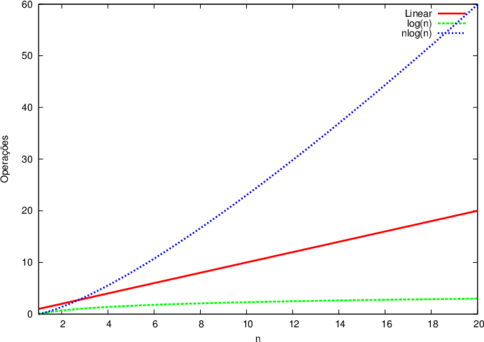
\includegraphics[height=0.6\paperheight]{pucrs-ec-poo-unidade_01-complexidade_de_algoritmos-laminas-grafico4.png}
	\end{figure}
\end{column}
\begin{column}{0.5\linewidth}
	\begin{figure}[h]
		\centering
		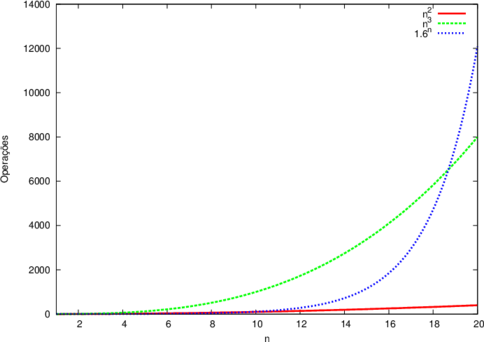
\includegraphics[height=0.6\paperheight]{pucrs-ec-poo-unidade_01-complexidade_de_algoritmos-laminas-grafico5.png}
	\end{figure}
\end{column}
\end{columns}

\end{frame}

%-------------------------------------------------------
\begin{frame}\frametitle{Funções}
\begin{itemize}
	\item Um problema é dividido em funções/métodos
	\begin{itemize}
		\item Cada função/método tem um ``custo'' diferente
		\item Estes custos são somados para determinar o custo total para solução do problema
	\end{itemize}
\end{itemize}
\end{frame}

%-------------------------------------------------------
\begin{frame}\frametitle{Exercício 1}
\begin{itemize}
	\item Dois algoritmos para resolver o mesmo problema\\
$f_{1}(n) = 2n^2 + 5n$ operações\\
$f_{2}(n) = 500n + 4000$ operações
	\item Considere o número de operações de cada um para diferentes valores de $n$ (por exemplo, $n = 10$ e $n = 1000$)
	\item Qual é a melhor solução?
\end{itemize}
\end{frame}

%-------------------------------------------------------
\begin{frame}[fragile]\frametitle{Exercício 2} % Fonte: https://create.kahoot.it/details/2e37a282-4d9d-4902-8afc-9b827ed393fc
Qual a complexidade do algoritmo abaixo?
{\scriptsize
\begin{verbatim}
v[1..N] : inteiro
maximo = 0
for (i=1; i<=n; ++i)
    sum = 0   // sum = somatorio de x[i..j]
    for (j = i; j <= n; ++j)
        sum += x[j]
    maximo = max(maximo,sum)
\end{verbatim}
}
\begin{enumerate}[A]
	\item $O(n)$
	\item $O(n^2)$ % CERTA
	\item $O(n \log 2n)$
	\item $O(2n)$
\end{enumerate}
\end{frame}

%-------------------------------------------------------
\begin{frame}[fragile]\frametitle{Exercício 3} % Fonte: https://create.kahoot.it/details/2e37a282-4d9d-4902-8afc-9b827ed393fc
Qual a complexidade do algoritmo abaixo?
{\scriptsize
\begin{verbatim}
int busca(v[1..N] : inteiro, elem : inteiro)
    for (i = 1; i <= n; i++)
        if (elem == v[i])
           return i // elemento encontrado no indice i
    return -1  // elemento NAO encontrado
\end{verbatim}
}
\begin{enumerate}[A]
	\item $O(n)$ % CERTA
	\item $O(n^2)$
	\item $O(n \log 2n)$
	\item $O(2n)$
\end{enumerate}
\end{frame}

\begin{comment}
%-------------------------------------------------------
\begin{frame}\frametitle{Funções}
\begin{itemize}
	\item 
Exercício:
https://kahoot.com/

\end{comment}

%=======================================================
\section{Créditos}

%-------------------------------------------------------
\begin{frame}\frametitle{Créditos}
\begin{itemize}
	\item Estas lâminas contêm trechos de materiais criados e disponibilizados pela professora Isabe Harb Manssour.
\end{itemize}
\end{frame}

%-------------------------------------------------------
\end{document}

